% @Author: Zihan Wu
% @Date:   2024-04-20 21:21:00
% @Last Modified by:   Zihan Wu
% @Last Modified time: 2024-04-30 23:52:00
% sectionis/method.tex

\section{Mathematical Formulation and Problem Statement}\label{sec:formula}

\subsection{Mathematical Formulation of Co-clustering}
Co-clustering groups rows and columns of a data matrix $\mathbf{A} \in \mathbb{R}^{M \times N}$, where $M$ is the number of features and $N$ is the number of samples. Each element $a_{ij}$ represents the $i$-th feature of the $j$-th sample. The goal is to partition $\mathbf{A}$ into $k$ row clusters and $d$ column clusters, creating $k \times d$ homogeneous submatrices $\mathbf{A}_{I, J}$.

When optimally reordered, $\mathbf{A}$ forms a block-diagonal structure where each block is a co-cluster with high internal similarity. Row and column labels are \( u \in \{1,\dots,k\}^M \) and \( v \in \{1,\dots,d\}^N \). Indicator matrices \( R \in \mathbb{R}^{M \times k} \) and \( C \in \mathbb{R}^{N \times d} \) assign rows and columns to clusters, ensuring unique assignments.

\subsection{Problem Statement}
This paper aims to develop a method to efficiently and accurately identify co-clusters $\mathbf{A}_{I, J}$ in large datasets. These co-clusters should exhibit uniformity, consistency, or specific patterns. Proper identification and categorization of these patterns are crucial for understanding complex data structures. Our method enhances co-clustering detection capabilities, improving efficiency and precision for large-scale data challenges.

\begin{table*}[h]
    \centering
    \begin{tabular}{c|p{10cm}}
        \hline
        \textbf{Symbol}        & \textbf{Description}                                                                                                           \\
        \hline
        $\mathbf{A}$           & Data matrix of dimensions $M \times N$, where $M$ is the number of rows (features) and $N$ is the number of columns (samples). \\
        $a_{ij}$               & Element at the $i$-th row and $j$-th column of matrix $\mathbf{A}$.                                                            \\
        $I, J$                 & Indices of rows and columns selected for co-clustering.                                                                        \\
        $\mathbf{A}_{I, J}$    & Submatrix containing the rows indexed by $I$ and columns by $J$.                                                               \\
        $R, C$                 & Indicator matrices for row and column cluster assignments.                                                                     \\
        $\phi_i, \psi_j$       & Block sizes in rows and columns, respectively.                                                                                 \\
        $s_i^{(k)}, t_j^{(k)}$ & Minimum row and column sizes of co-cluster $C_k$ in block $B_{(i,j)}$.                                                         \\
        $P(\omega_k)$          & Probability of failure to identify co-cluster $C_k$.                                                                           \\
        $T_p$                  & Number of sampling times or iterations in the probabilistic model.                                                             \\
        \hline
    \end{tabular}
    \caption{Notations used in the mathematical formulation of co-clustering}
    \label{tab:notations}
\end{table*}

\section{The Scalable Co-clustering Method}
\label{sec:method}
\subsection{Overview}

% insert workflow.png here
\begin{figure*}[htbp]
    \centering
    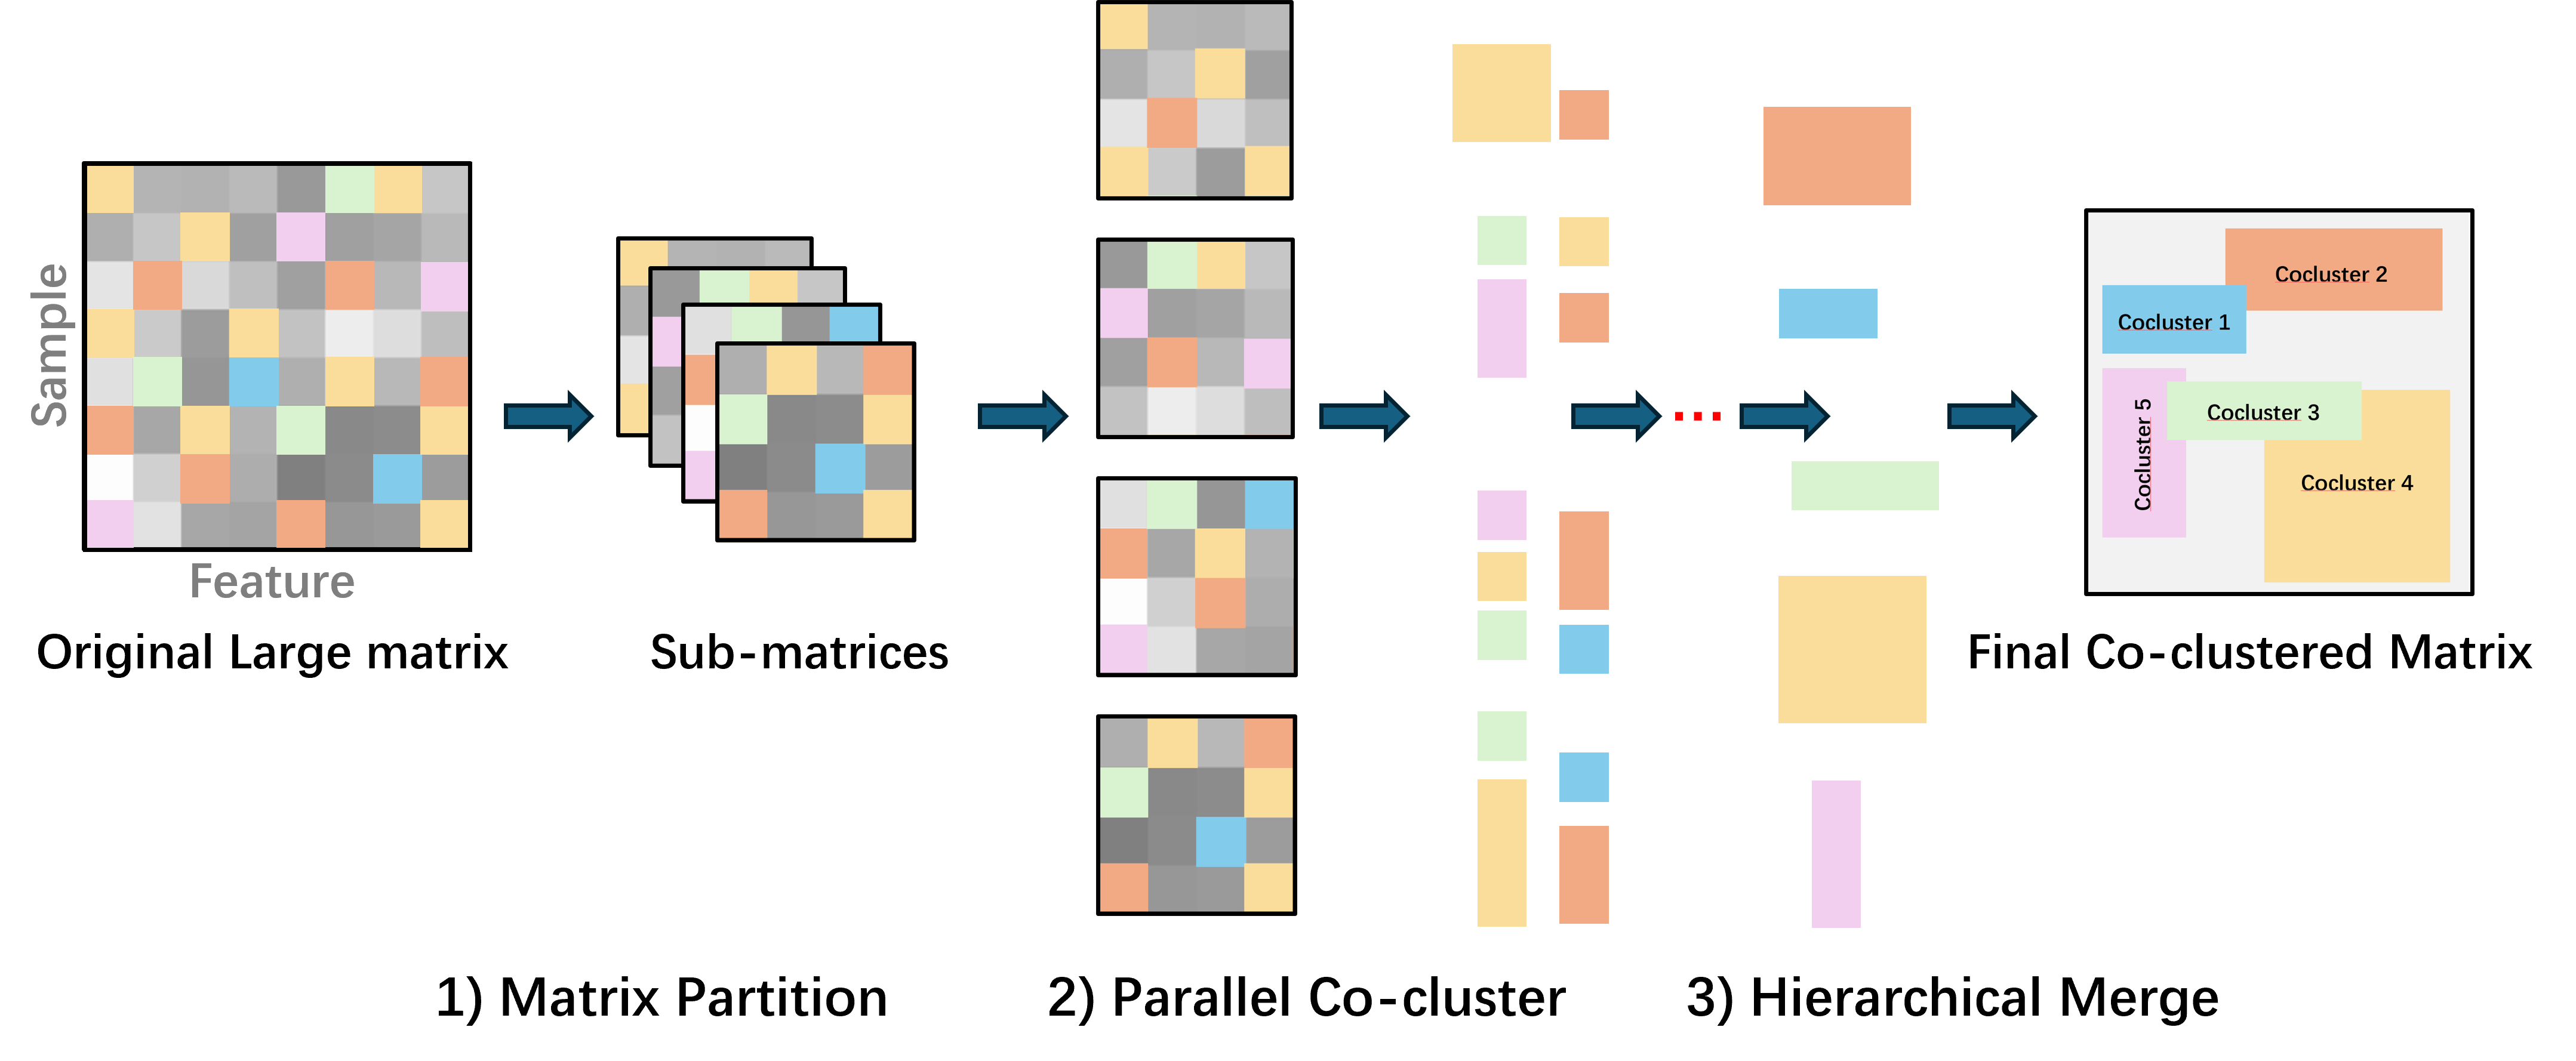
\includegraphics[width=0.8\linewidth]{workflow.png}
    \caption{Workflow of our proposed AHPM for large matrices.}
    \label{fig:workflow}
\end{figure*}
This paper presents a novel and scalable co-cluster method specifically designed for large matrices, as shown in \Cref{fig:workflow}. This method applies a probabilistic model-based optimal partitioning algorithm, which not only predicts the ideal number and sequence of partitions for maximizing computational efficiency but also ensures the effectiveness of the co-clustering process.

Our method involves partitioning large matrices into smaller, manageable submatrices. This strategic partitioning is meticulously guided by our algorithm to facilitate parallel processing. By transforming the computationally intensive task of co-clustering a large matrix into smaller, parallel tasks, our approach significantly reduces computational overhead and enhances scalability.

Following the partitioning, each submatrix undergoes a co-clustering process. This is implemented via the application of Singular Value Decomposition (SVD) and $k$-means clustering on the resulting singular vectors. This pivotal step ensures the adaptability of our method, allowing our algorithm to tailor its approach to the unique characteristics of each submatrix, thus optimizing clustering results.

Furthermore, our method integrates a novel hierarchical merging strategy that combines the co-clustering results from all submatrices. This integration provides more fine-grained insight into each submatrix and enhances the overall accuracy and reliability of the co-clustering results. Our method, validated and optimized through a comprehensive process, showed efficiency in handling large-scale datasets that were never reached before.


\subsection{Large Matrix Partitioning}
% Description of the matrix partitioning process and criteria for partitioning.
The primary challenge in co-clustering large matrices is the risk of losing co-clusters when the matrix is partitioned into smaller submatrices. To address this, we introduce an optimal partitioning algorithm underpinned by a probabilistic model. This model is meticulously designed to navigate the complexities of partitioning, ensuring that the integrity of co-clusters is maintained even as the matrix is divided. The objective of this algorithm is twofold: to determine the optimal partitioning strategy that minimizes the risk of fragmenting significant co-clusters and to define the appropriate number of repartitioning iterations needed to achieve a desired success rate of co-cluster identification.

\subsubsection{Partitioning and Repartitioning Strategy based on the Probabilistic Model}
Our probabilistic model serves as the cornerstone of the partitioning algorithm. It evaluates potential partitioning schemes based on their ability to preserve meaningful co-cluster structures within smaller submatrices. The model operates under the premise that each atom-co-cluster (the smallest identifiable co-cluster within a submatrix) can be identified with a probability $p$. This probabilistic model allows us to estimate the likelihood of successfully identifying all relevant co-clusters across the partitioned submatrices.

In the scenario where the matrix $A$ is partitioned into $m \times n$ blocks, each block has size $\phi_i \times \psi_j$, that is, $M=\sum_{i=1}^m \phi_i$ and $N=\sum_{j=1}^n \psi_j$, the joint probability of $M_{(i,j)}^{(k)}$ and $N_{(i,j)}^{(k)}$ are
\begin{equation}
    \label{eq:joint_probability}
    \begin{split}
        P(M_{(i,j)}^{(k)} & < T_m, N_{(i,j)}^{(k)} < T_n)                                                                           \\
                          & = \sum_{\alpha=1}^{T_m-1} \sum_{\beta=1}^{T_n-1} P(M_{(i,j)}^{(k)} = \alpha) P(N_{(i,j)}^{(k)} = \beta) \\
                          & \le \exp[-2 (s_i^{(k)})^2 \phi_i + -2 (t_j^{(k)})^2 \psi_j]
    \end{split}
\end{equation}
where $s_i^{(k)}$ and $t_j^{(k)}$ are the minimum row and column sizes of co-cluster $C_k$ in block $B_{(i,j)}$, the size of the co-cluster $C_k$ is $M^{(k)} \times N^{(k)}$, and $M^{(k)}$ and $N^{(k)}$ are the row and column sizes of co-cluster $C_k$, respectively.

% the size of co-cluster Ck∈RM(k)×N(k)C_k \in \mathbb{R}^{M^{(k)} \times N^{(k)}} that falls into block B(i,j)B_{(i,j)} is M(k)(i,j)×N(k)(i,j)M_{(i,j)}^{(k)} \times N_{(i,j)}^{(k)};

Thus, the probability of identifying all co-clusters is given by

\begin{equation}
    \begin{split}
        P(\omega_k) & \le \exp \left\{ -2 [\phi m (s^{(k)})^2 + \psi n (t^{(k)})^2] \right\},
    \end{split}
\end{equation}
and
\begin{equation}
    \begin{split}
        P & = 1 - P(\omega_k)^{T_p}                                                                                                       \\
          & \ge 1 - \exp \left\{ -2 T_p [\phi m (s^{(k)})^2 + \psi n (t^{(k)})^2] \right\} \label{eq:prob_of_identifying_all_co_clusters}
    \end{split}
\end{equation}
where $P(\omega_k)$ is the probability of the failure of identifying co-cluster $C_k$, $T_p$ is the number of sampling times, $\phi$ and $\psi$ are the row and column block sizes, and $s^{(k)}$ and $t^{(k)}$ are the minimum row and column sizes of co-cluster $C_k$.

\Cref{eq:prob_of_identifying_all_co_clusters} is central to our algorithm for partitioning large matrices, providing a probabilistic model to optimize our strategy and preserve co-cluster integrity. It quantifies the likelihood of identifying all relevant co-clusters within partitioned blocks, helping mitigate risks of fragmentation.

Using \eqref{eq:prob_of_identifying_all_co_clusters}, we can establish a constraint between the repartitioning time $T_r$ and the partition solution $Part$, ensuring adherence to a predetermined success rate and minimizing the risk of co-cluster fragmentation. Details of these constraints are discussed in the appendix due to space limitations.

\subsubsection{Optimization and Computational Efficiency}
Optimizing the partitioning process for computational efficiency is crucial in both academic and industrial applications. Our optimization strategy focuses on minimizing running time without compromising the integrity of co-cluster identification.

We assess various partitioning configurations to balance computational resource allocation and success rate adherence. By evaluating the impact of different schemes, we identify strategies that meet co-clustering criteria and optimize resource use.

To ensure efficiency without sacrificing quality, we introduce conditions for optimization that maintain co-cluster identification success. These conditions provide a mathematical basis for balancing computational efficiency and co-cluster identification fidelity.

The optimization must satisfy:
\begin{equation}
    \label{eq:optimization_condition}
    T_p = \text{argmin}_{T_p} \{
    1 - \exp \{ -2 T_p [\phi m (s^{(k)})^2 + n (t^{(k)})^2] \} \ge P_{\text{thresh}} \}
\end{equation}

Adhering to these conditions ensures our optimization efforts preserve the effectiveness of co-cluster discovery, making the partitioning algorithm fast, efficient, and robust across various datasets and challenges.

\subsection{Co-clustering on Small Submatrices}
% Detailed method for co-clustering within each of the submatrices.

\subsubsection{Atom-co-clustering Algorithm}
Our framework, which encompasses both partitioning and ensembling, offers remarkable flexibility, allowing it to be compatible with a wide range of atom-co-clustering methods. For the sake of making this paper comprehensive and self-contained, we provide an introduction to the atom-co-cluster method herein. The only requirement for an atom-co-clustering method to be compatible with our framework is that it must be able to identify co-clusters under a given criterion with a probability $p$, or more relaxed conditions, has a lower bound estimate of the probability of identifying co-clusters equipped with a validation mechanism.

\subsubsection{Graph-based Spectral Co-clustering Algorithm}
Spectral co-clustering (SCC) is widely used for high-dimensional data due to its effectiveness in partitioning data into clusters based on graph Laplacian eigenvectors \cite{vonluxburg2007TutorialSpectralClustering}. SCC constructs a bipartite graph $G=(U,V,E)$ from the data matrix $A$, where $U$ and $V$ represent rows and columns, respectively, and $E$ are weighted edges indicating relationships.

The Laplacian matrix $L = D - W$ is computed, where $D$ is the degree matrix, and $W$ is the weighted adjacency matrix. Eigenvectors of the smallest positive eigenvalues of $L$ are used to partition the graph. The normalized matrix $A_n = D^{-1/2} A D^{-1/2}$ is factorized using singular value decomposition (SVD), and the resulting singular vectors are used for clustering.

For co-clustering, we apply $k$-means to the rows of the matrix formed by stacking the left and right singular vectors of $A_n$. This method effectively identifies clusters in high-dimensional data, making it suitable for our framework \cite{dhillon2001CoclusteringDocumentsWords}.

\begin{algorithm}[ht]
    \caption{Optimal Matrix Partition and Hierarchical Co-cluster Merging Method}\label{alg:method}
    \begin{algorithmic}[1]
        \REQUIRE{Data matrix $A \in \mathbb{R}^{M \times N}$, Co-cluster set $C = \{C_k\}_{k=1}^K$, Block sizes $\{\phi_i\}_{i=1}^m$, $\{\psi_j\}_{j=1}^n$, Thresholds $T_m$, $T_n$, Sampling times $T_p$, Probability threshold $P_\text{thresh}$;}
        \ENSURE{Co-clustered result $\mathcal{C}$;}
        \STATE Initialize block set $B = \{B_{(i,j)}\}_{i=1}^m,_{j=1}^n$ on $\phi_i$ and $\psi_j$
        \STATE Calculate $s^{(k)}$ and $t^{(k)}$ for each co-cluster $C_k$
        \FOR{$k=1$ to $K$}
        \STATE Calculate $P(\omega_k)$ for co-cluster $C_k$
        \IF{$P(\omega_k) < P_{thresh}$}
        \STATE Partition matrix $A$ into blocks $B$ and perform co-clustering
        \STATE Aggregate co-clustered results from each block
        \ENDIF
        \ENDFOR
        \RETURN Aggregated co-clustered result $\mathcal{C}$
    \end{algorithmic}
\end{algorithm}

\begin{table*}[!htbp]
    \centering
    \caption{Comparison of Running Times (in seconds) for Various Co-clustering Methods on Selected Datasets.}
    \label{tab:running-time}
    \begin{tabular}{@{} l cccc @{}}
        \toprule
        Dataset     & SCC \cite{dhillon2001CoclusteringDocumentsWords} & PNMTF \cite{chen2023ParallelNonNegativeMatrix} & \textbf{AHPM-SCC} & \textbf{AHPM-PNMTF} \\
        \midrule
        Amazon 1000 & 64545.2                                          & 303.7                                          & 112.5             & 242.8               \\
        CLASSIC4    & *                                                & 17,810                                         & 22,894            & 3,028               \\
        RCV1-Large  & *                                                & 277,092                                        & *                 & 208,048             \\
        % ... more rows here
        \bottomrule
    \end{tabular}
    \begin{tablenotes}
        \small
        \item Notes: * indicates that the method cannot process the dataset because the dataset size exceeds the processing limit.
    \end{tablenotes}
\end{table*}

\begin{table*}[!htbp]
    \centering
    \caption{NMIs and ARIs Scores for Various Co-clustering Methods on Selected Datasets.}
    \label{tab:evaluation-metrics}
    \begin{tabular}{@{} l c cccc @{}}
        \toprule
        \multirow{2}{*}{Dataset}     & \multirow{2}{*}{Metric} & \multicolumn{4}{c}{Compared Methods}                                                                                                        \\
        \cmidrule{3-6}
                                     &                         & SCC \cite{dhillon2001CoclusteringDocumentsWords} & PNMTF \cite{chen2023ParallelNonNegativeMatrix} & \textbf{AHPM-SCC} & \textbf{AHPM-PNMTF} \\
        \midrule
        \multirow{2}{*}{Amazon 1000} & NMI                     & 0.9223                                           & 0.6894                                         & 0.8650            & 0.6609              \\
                                     & ARI                     & 0.7713                                           & 0.6188                                         & 0.7763            & 0.6057              \\
        \multirow{2}{*}{CLASSIC4}    & NMI                     & *                                                & 0.5944                                         & 0.7676            & 0.6073              \\
                                     & ARI                     & *                                                & 0.4523                                         & 0.5845            & 0.4469              \\
        \multirow{2}{*}{RCV1-Large}  & NMI                     & *                                                & 0.6519                                         & 0.8349            & 0.6348              \\
                                     & ARI                     & *                                                & 0.5383                                         & 0.7576            & 0.5298              \\
        % ... more rows here
        \bottomrule
    \end{tabular}
    \begin{tablenotes}
        \small
        \item Notes: * indicates that the method cannot process the dataset because the dataset size exceeds the processing limit.
    \end{tablenotes}
\end{table*}

\subsection{Hierarchical Co-cluster Merging}
% Explanation of how co-clustered results from submatrices are aggregated.

With the co-clustering results from each submatrix in hand, the next step is to merge these results to form the final co-clustered output. This merging process employs a hierarchical strategy that starts with the most closely related clusters, gradually integrating broader groups to maintain consistency and reduce redundancy. Throughout this process, the algorithm assesses and recalibrates the similarity thresholds necessary to ensure clusters are combined appropriately, thus accommodating the diverse nature of the data. By iteratively refining the merging criteria, the framework can adaptively reconcile differences among submatrix clusters, resulting in a robust and coherent final clustering solution that reflects the inherent structure of the entire dataset. This approach not only preserves the detailed information within each subcluster but also enhances the overall clustering accuracy and reliability.

\subsection{Algorithmic Description}
% Step-by-step algorithmic description of the process in pseudocode.
Our proposed  Optimal Matrix Partition and Hierarchical Co-cluster Merging Method is outlined in Algorithm \ref{alg:method}. The algorithm
is an advanced algorithm designed for efficient co-clustering of large data matrices. The algorithm begins by initializing a block set based on predetermined block sizes. For each co-cluster in the given set, the algorithm calculates specific values $s^{(k)}$ and $t^{(k)}$, which are then used to determine the probability $P(\omega_k)$ of each co-cluster. If this probability falls below a predefined threshold $P_{\text{thresh}}$, the algorithm partitions the data matrix $A$ into blocks $B$ and performs co-clustering on these blocks. This step is crucial for managing large datasets by breaking them down into smaller, more manageable units. After co-clustering, the results from each block are aggregated to form the final co-clustered result $\mathcal{C}$. The algorithm's design allows for a flexible and efficient approach to co-clustering, particularly suited to datasets with high dimensionality and complexity.
